\documentclass[a4paper,12pt]{report}
\usepackage{graphicx} % for including images
\usepackage{hyperref} % for adding links
\usepackage{fancyhdr} % for customizing the header and footer
\usepackage{ragged2e} % for left-aligning text on the title page
\usepackage{multicol} % for placing signatures on the same line
\usepackage{float}
\usepackage{svg}
\pagestyle{fancy}
\fancyhf{}
\fancyhead[L]{Summer Practice Report}
\fancyfoot[C]{\thepage}

\begin{document}

% Title Page with Image
\begin{titlepage}
    \centering
    % Include the image at the top of the cover page
    
\includegraphics[width=1\textwidth]{cover_image.png} % Adjust width as needed
    
    \vspace*{1cm}

    \Huge
    \textbf{SUMMER PRACTICE REPORT}

    \vspace{1.5cm}

    \LARGE
    \textbf{CENG300}
    
    \vfill

    % Left-align the details part and make them bold with smaller font size
    \RaggedRight
    \large
    \textbf{STUDENT NAME:} Burak YILDIZ \\
    \textbf{ORGANIZATION NAME:} Intertech Bilgi İşlem ve Pazarlama Tic. A.Ş \\
    \textbf{ADDRESS:} Sanayi Mah Teknopark Bulvarı 1/3 C Blok Kurtköy İstanbul \\
    \textbf{START DATE:} 08.07.2024 \\
    \textbf{END DATE:} 05.08.2024 \\
    \textbf{TOTAL WORKING DAYS:} 20 \\
    \textbf{TOTAL WORKING DAYS:} 20 \\
    \vfill

    % Left and right-aligned signatures
    \begin{multicols}{2}
        \raggedright \textbf{STUDENT’S SIGNATURE} \\
        \raggedleft \textbf{ORGANIZATION APPROVAL}
    \end{multicols}

    \vfill
\end{titlepage}

\tableofcontents
\newpage

% Section 1: Introduction
\chapter{Introduction}
This report provides an overview of the summer practice I completed at Intertech Bilgi İşlem ve Pazarlama Tic. A.Ş, a subsidiary of DenizBank, from 08.07.2024 to 05.08.2024. Intertech is a leading technology company specializing in providing innovative solutions in the financial sector. The company focuses on delivering software solutions that enhance operational efficiency and customer service within the banking industry.

The summer practice started with a series of training sessions, where we were introduced to various tools and technologies relevant to the projects we would later undertake. These trainings covered multiple fields, including business analysis, agile, AI, Flask, Figma, ReactJS and mobile frontend. These sessions provided a solid foundation for understanding the technical environment at Intertech, equipping me and my peers with the necessary skills to contribute effectively to our projects.

Following the training, we were divided into groups and tasked with completing projects that followed the Agile methodology. My group’s project was to design a webapp and develop a financial advisor bot, powered by Azure OpenAI services. This bot aimed to assist users by offering personalized financial advice based on real-time data analysis.

Github repo for the project : https://github.com/samemrecebi/finantial-advisor

Throughout the project, I was actively involved in various aspects of the development process. My contributions included:

\begin{itemize}
    \item Backend development: I worked on setting up the server-side components and ensuring data integration with the bot’s features.
    \item Frontend development: I contributed to the user interface of mainly the chat-screen, ensuring a seamless and user-friendly experience for customers interacting with the bot.
    \item Prompt engineering: I utilized Azure OpenAI services to craft and optimize prompts for the bot, ensuring it generated relevant and accurate responses based on the user's queries.
\end{itemize}

The rest of this report is structured as follows:
\begin{itemize}
    \item Chapter 2 covers detailed information about the project, divided into the analysis, design, implementation, and testing phases.
    \item Chapter 3 provides observations on the structure and methodologies of the organization.
    \item Chapter 4 concludes with a summary of the overall experience and key learnings.
\end{itemize}

Throughout the report, relevant screenshots and figures are included to illustrate the technical aspects and progress of the project. 


% Section 2: Information about the Project
\chapter{Information about the Project}

\section{Analysis Phase}
The analysis phase of the financial advisor bot project began with a thorough examination of the project's objectives and the expected functionalities of the bot. The primary goal was to create a bot capable of offering personalized financial advice to users by analyzing real-time data. This required identifying the data sources, understanding the core financial queries users might ask, and ensuring that the bot could process and respond to those queries effectively.

\subsection*{Problem Identification}
During the initial analysis, we identified several key challenges:
\begin{itemize}
    \item \textbf{Data Integration:} One of the main challenges was determining how to integrate various financial data sources into the bot. The data needed to be accurate, up-to-date, and securely processed to ensure the quality of the financial advice provided.
    \item \textbf{User Query Understanding:} Another challenge was ensuring that the bot could interpret a wide range of user queries. This required us to develop a system for understanding natural language inputs effectively, which involved creating a robust prompt design using Azure OpenAI.
    \item \textbf{Response Accuracy:} Ensuring that the bot's responses were not only relevant but also accurate was crucial. This was especially challenging when dealing with complex financial concepts and up to date data.
\end{itemize}

\subsection*{Methods Followed}
To address these challenges, the following steps were taken:
\begin{itemize}
    \item \textbf{Data Source Evaluation:} We started by identifying and evaluating various financial data providers, ensuring that the data sources were reliable, real-time, and aligned with the bot's needs. This involved both internal data from the organization and third-party APIs for market data. We have used DenizYatirim's daily bulletins and various API's for currency rates and stock exchange rates.
    \item \textbf{User Requirement Gathering:} We conducted interviews with stakeholders and potential users to gather insights into the most common financial questions they might ask. Based on this, we developed a list of high-priority features for the bot.
    \item \textbf{Prompt Engineering:} We utilized Azure OpenAI’s capabilities to design and test prompts that would allow the bot to accurately interpret and respond to financial queries. This included experimenting with different prompt formats and tuning the responses based on test cases.
\end{itemize}

\subsection*{Solutions Implemented}
The following solutions were implemented to overcome the identified challenges:
\begin{itemize}
    \item For data integration, we used secure API connections to pull data from trusted sources. To ensure data accuracy, real-time synchronization methods were applied.
    \item For user query understanding, we developed a prompt structure that allowed the bot to handle both simple and complex queries by recognizing key financial terms.
    \item For response accuracy, we continuously tested the bot’s responses using various test queries, refining the model's performance through prompt adjustments and data validation.
\end{itemize}

\subsection*{Evaluation of Project Management}
The project followed the Agile methodology, which allowed for iterative development and continuous feedback. During the analysis phase, the flexibility of Agile enabled our team to adapt to new challenges as they arose, such as changes in user requirements or data availability.

\textbf{Strengths:}
\begin{itemize}
    \item The Agile methodology facilitated effective collaboration between team members, ensuring that we could address issues promptly and efficiently.
    \item Regular feedback from stakeholders during sprint reviews helped refine our understanding of the project requirements.
\end{itemize}

\textbf{Areas for Improvement:}
\begin{itemize}
    \item Initial data source evaluations took longer than expected, which delayed some parts of the analysis phase.
    \item More upfront testing of user queries could have been beneficial, as some prompt designs needed significant adjustment after initial testing.
\end{itemize}

\subsection*{Figures and Screenshots}
In this section, I will include relevant screenshots to illustrate the analysis process, such as the activity diagram and the scope canvas.

\begin{figure}[H]
    \centering
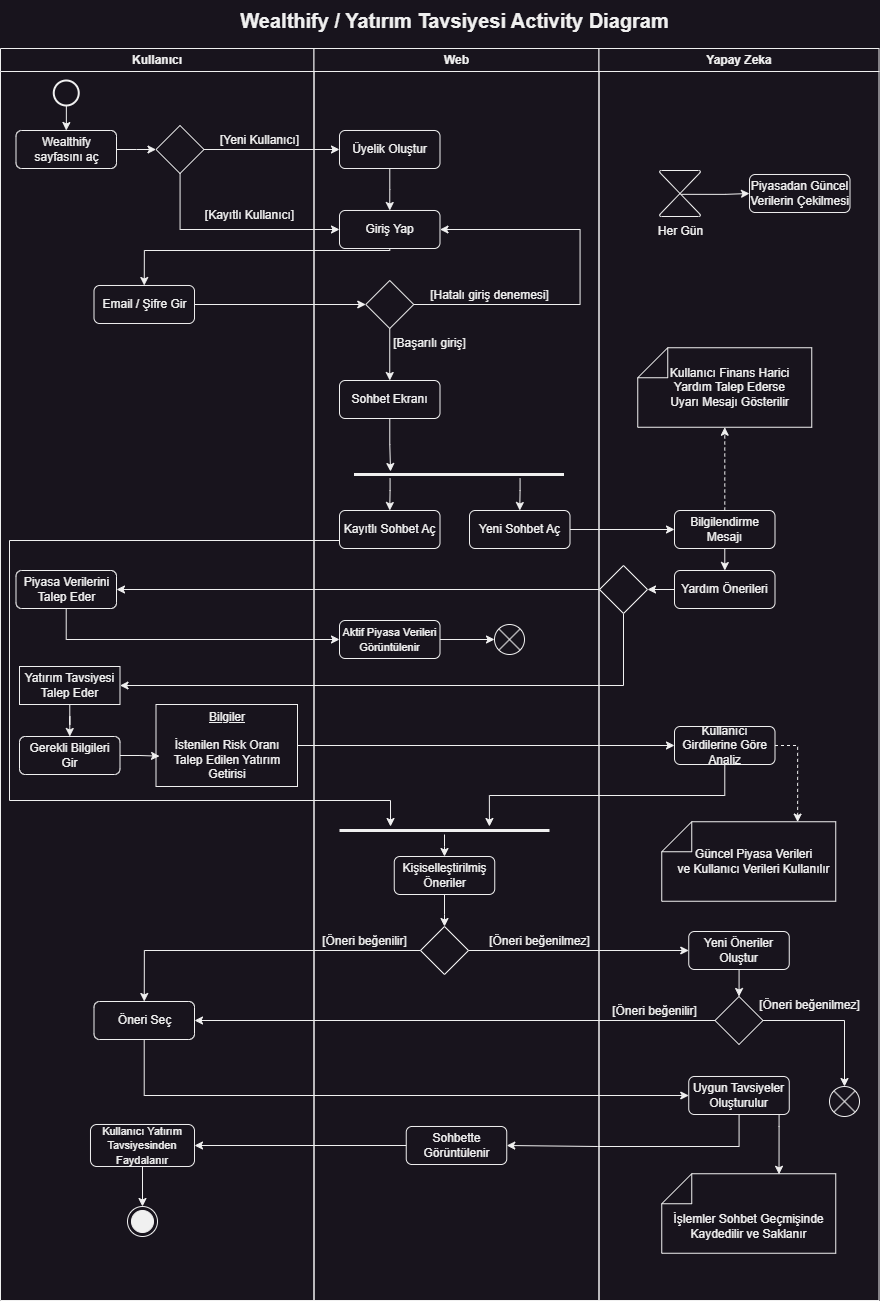
\includegraphics[width=0.8\textwidth]{activity_diagram.png}
\caption{Activity Diagram for Wealthify}
\end{figure}

\begin{figure}[H]
    \centering
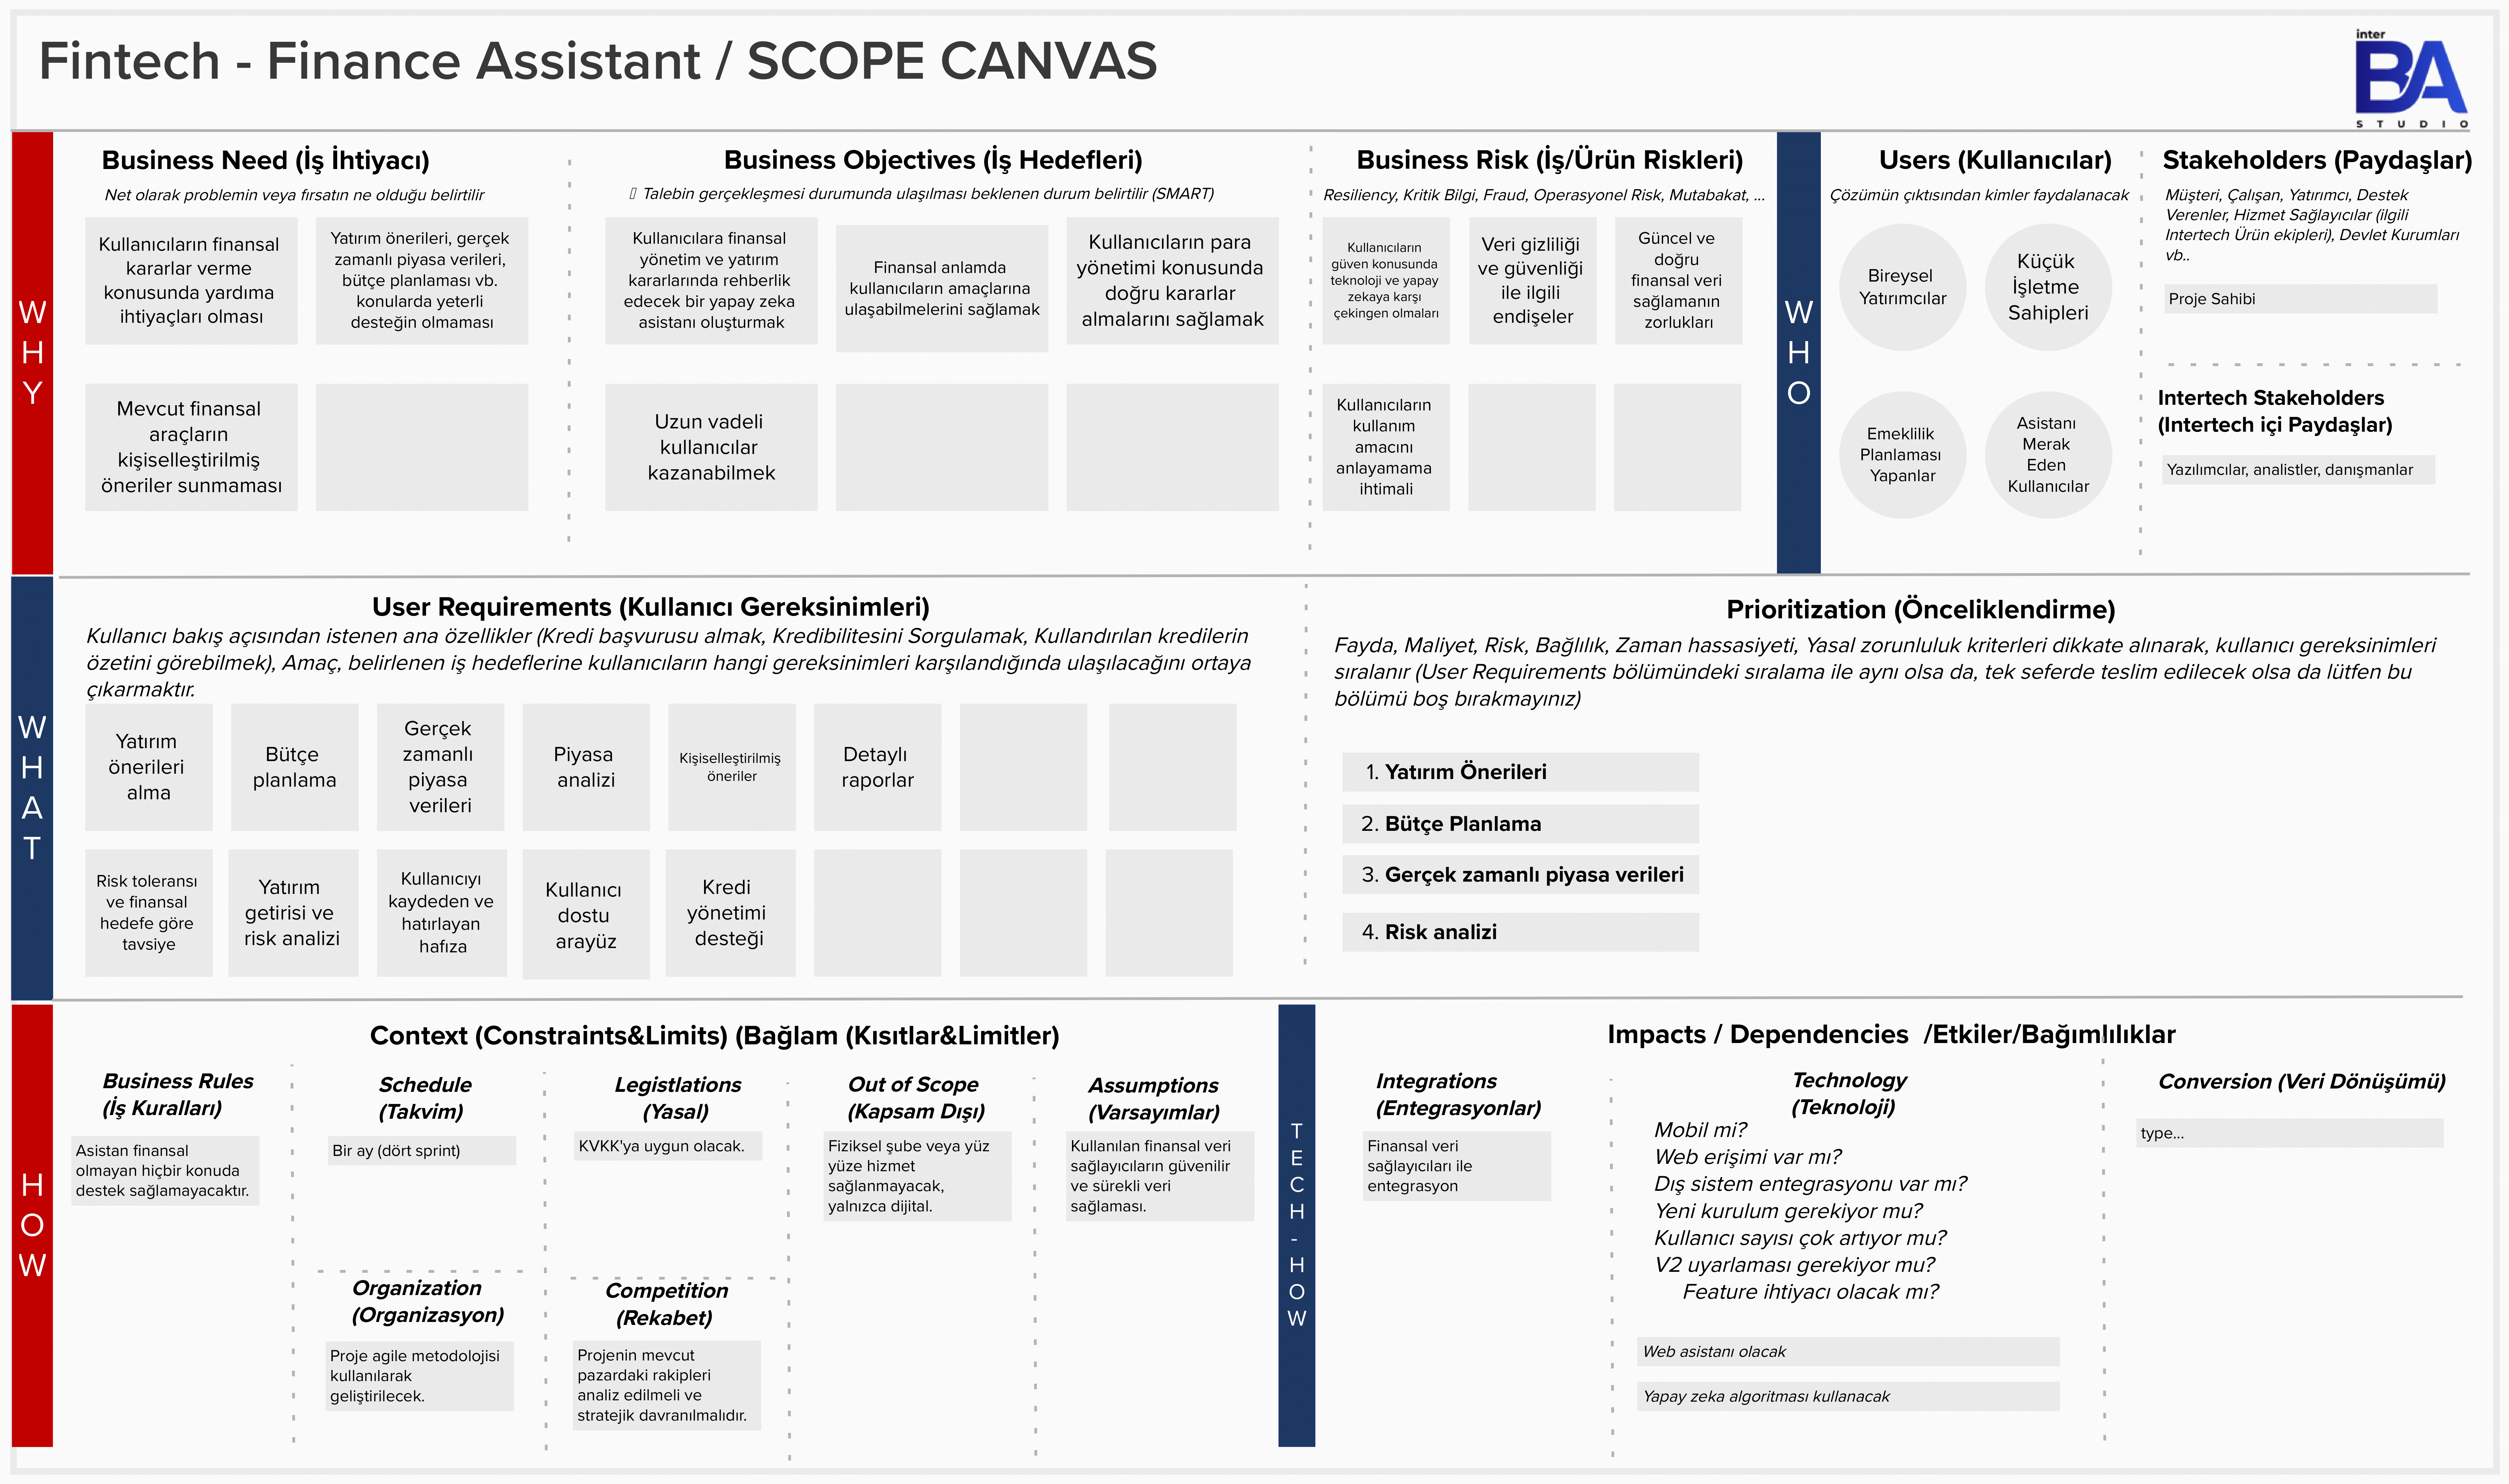
\includegraphics[scale = 0.16]{scope_canvas.png}
\caption{Scope Canvas for Fintech (later to be renamed as Wealthify)}
\end{figure}

\section{Design Phase}
The design phase focused on translating the requirements gathered during the analysis phase into a structured solution. This involved designing the system architecture for the financial advisor bot, outlining the interaction between different components (backend, frontend, and Azure OpenAI services), and ensuring a scalable, efficient, and user-friendly design.

\subsection*{System Architecture}
The bot's architecture was designed to ensure seamless interaction between the backend (which handled data processing and storage), the frontend (the user interface), and Azure OpenAI services (for natural language processing). The architecture included:
\begin{itemize}
    \item \textbf{Backend:} The backend was designed to handle API requests, data processing, and integration with third-party financial data sources. It also managed the logic for interacting with Azure OpenAI.
    \item \textbf{Frontend:} The frontend was designed with simplicity and user experience in mind. We aimed to create a responsive interface that allowed users to input queries easily and receive clear, accurate responses.
    \item \textbf{Azure OpenAI Integration:} The OpenAI service was integrated into the architecture to process and generate responses based on user input. It was essential to ensure that this integration was both fast and reliable, providing real-time advice to users.
\end{itemize}

\subsection*{Challenges in Design}
The design phase presented several challenges:
\begin{itemize}
    \item \textbf{Scalability:} One of the major design challenges was ensuring that the bot could scale to accommodate multiple users querying the system simultaneously. We needed to ensure that both the backend and the OpenAI services could handle high loads without performance degradation.
    \item \textbf{User Interface Simplicity:} Designing an interface that was both simple and intuitive, while also providing sufficient information and options for advanced financial queries, required balancing ease of use with functionality.
    \item \textbf{Integration with Real-Time Data:} Ensuring that the bot could integrate and update real-time financial data from multiple sources presented a technical challenge in both design and implementation.
\end{itemize}

\subsection*{Solutions Implemented}
To overcome these challenges, the following design solutions were implemented:
\begin{itemize}
    \item For scalability, we used a microservices-based architecture for the backend. This allowed different parts of the system to be scaled independently based on demand. For instance, we could scale the financial data integration service separately from the Azure OpenAI service. For this feature we have used Kubernetes tests.
    \item For the user interface, we conducted multiple iterations of wireframe designs and usability tests. This allowed us to refine the layout and features based on user feedback, ensuring a simple and intuitive experience.
    \item For real-time data integration, we used a caching mechanism to temporarily store frequently requested financial data. This minimized the load on external APIs while ensuring that the data remained up-to-date.
\end{itemize}

\subsection*{Evaluation of the Design}
The design phase was highly collaborative, with regular design sprints and feedback sessions. This ensured that all stakeholders, including the development team and product owners, were aligned with the project's direction.

\textbf{Strengths:}
\begin{itemize}
    \item The microservices architecture provided a flexible and scalable solution for future expansion.
    \item The iterative design process for the user interface allowed for continual refinement based on user feedback, resulting in a highly user-friendly experience.
\end{itemize}

\textbf{Areas for Improvement:}
\begin{itemize}
    \item The initial integration of real-time data sources required more optimization than expected, as API rate limits and delays impacted performance.
    \item More attention could have been given to future-proofing the system for even larger data sets and user bases, though this was addressed later in the project.
\end{itemize}

\subsection*{Figures and Screenshots}
To illustrate the design phase, the following screenshots will be included:
\begin{figure}[H]
    \centering
    \includesvg[inkscapelatex=false, scale=0.7]{usecase_diagram.svg}
    \caption{Use Case Diagram for the project}
\end{figure}

\begin{figure}[H]
    \centering
    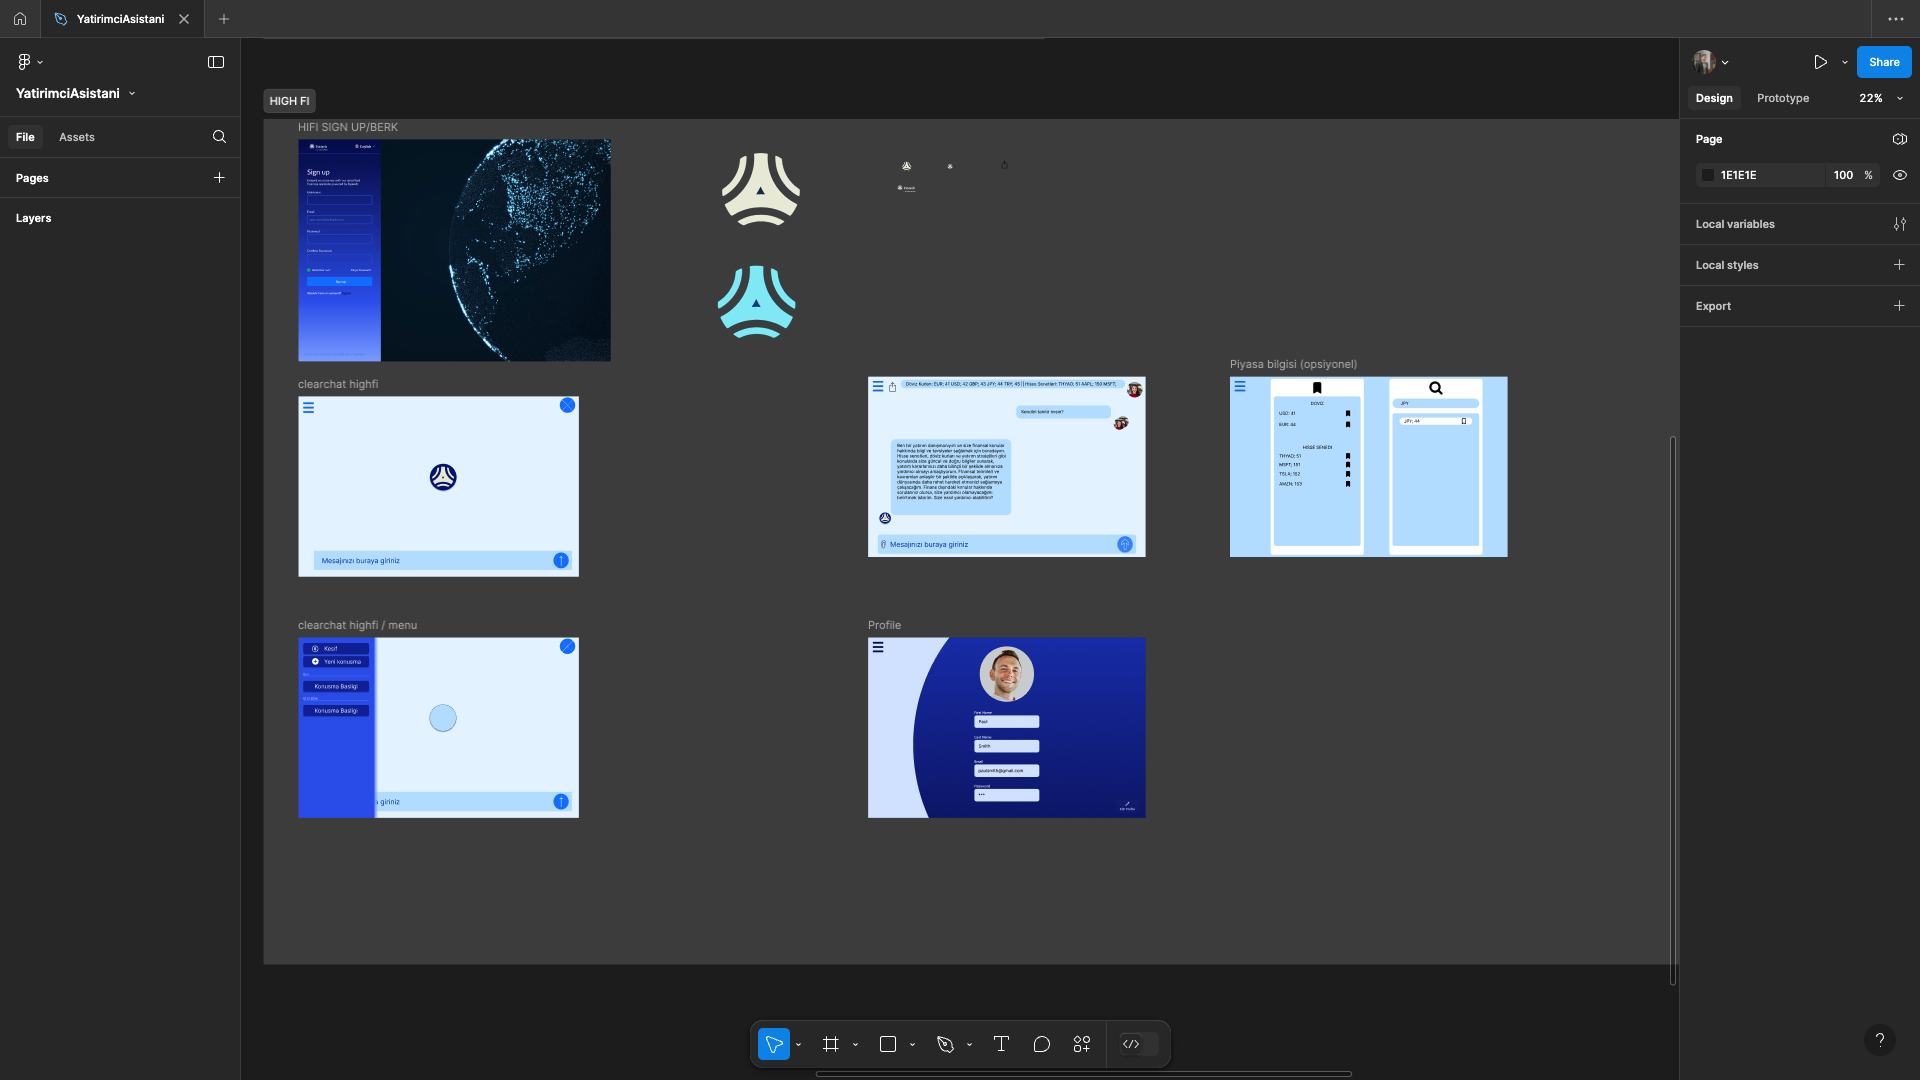
\includegraphics[width=0.8\textwidth]{figma_hifi.png}
    \caption{Wireframe Design of the User Interface}
    \label{fig:ui-wireframe}
\end{figure}


\section{Implementation Phase}
The implementation phase was focused on turning the design into a fully functional financial advisor bot. This involved developing the backend and frontend components, integrating Azure OpenAI services, and ensuring real-time data access.

\subsection*{Backend Development}
The backend development primarily involved setting up the server infrastructure, API integration, and business logic. The backend was responsible for handling user requests, fetching real-time data from financial APIs, processing the queries, and interacting with the Azure OpenAI service to generate responses. The key tasks during this phase included:
\begin{itemize}
    \item \textbf{API Integration:} Implemented API connections with third-party financial data providers to ensure the bot could access real-time data, such as stock prices, currency exchange rates, and market trends.
    \item \textbf{Data Processing:} Built data pipelines that processed incoming data to ensure it was accurate and formatted correctly for the bot to use.
    \item \textbf{Security:} Implemented security measures to protect sensitive financial data, such as encryption for data in transit and secure authentication methods for API access.
\end{itemize}

\subsection*{Frontend Development}
The frontend development aimed to create an intuitive user interface for customers to interact with the financial advisor bot. The frontend was designed using modern web development technologies to ensure a responsive and seamless user experience. The key tasks included:
\begin{itemize}
    \item \textbf{UI/UX Implementation:} Designed and developed a user-friendly interface based on the wireframes created during the design phase. This included input fields for user queries and dynamic sections to display financial data and advice.
    \item \textbf{Data Visualization:} Integrated data visualization features that allowed users to view financial trends, market data, and forecasts in easy-to-understand charts and graphs.
    \item \textbf{Responsive Design:} Ensured the frontend was responsive across different devices, allowing users to access the bot on both desktops and mobile devices.
\end{itemize}

\subsection*{Prompt Engineering}
One of the most critical aspects of the implementation phase was the integration of Azure OpenAI services, which required careful prompt engineering to ensure the bot could interpret and respond accurately to user queries. Key tasks in this area included:
\begin{itemize}
    \item \textbf{Prompt Design:} Developed a library of prompts that helped the bot understand various types of financial queries. These prompts were fine-tuned through multiple iterations to improve the accuracy of the bot’s responses.
    \item \textbf{Error Handling:} Implemented mechanisms for handling ambiguous or unclear queries, ensuring the bot could ask for clarification or provide alternative suggestions.
    \item \textbf{Continuous Testing and Tuning:} Conducted regular testing of the bot’s responses with real-world queries to fine-tune the prompts and improve response quality.
\end{itemize}

\subsection*{Challenges Encountered}
Several challenges were encountered during the implementation phase:
\begin{itemize}
    \item \textbf{Bot Response Accuracy:} Achieving high response accuracy was an iterative process. In the early stages, some responses from Azure OpenAI were too general or inaccurate, requiring significant prompt tuning and error-handling mechanisms.
    \item \textbf{Cross-Platform Compatibility:} Ensuring the frontend worked seamlessly across all devices, particularly mobile, presented challenges, especially when rendering complex data visualizations on smaller screens.
\end{itemize}

\subsection*{Solutions Implemented}
To overcome these challenges, the following solutions were implemented:
\begin{itemize}
    \item \textbf{Prompt Optimization:} Prompt engineering was continuously optimized, including the use of predefined templates for certain query types and leveraging OpenAI’s advanced capabilities to handle ambiguous queries.
    \item \textbf{Mobile Optimization:} The frontend was optimized for mobile use by ensuring that all components were responsive and that data visualizations adapted to smaller screen sizes without losing clarity.
\end{itemize}

\subsection*{Figures and Screenshots}
This section will include screenshots demonstrating the implementation phase, such as backend API calls, frontend user interface elements, and examples of prompt designs.

\begin{figure}[H]
    \centering
    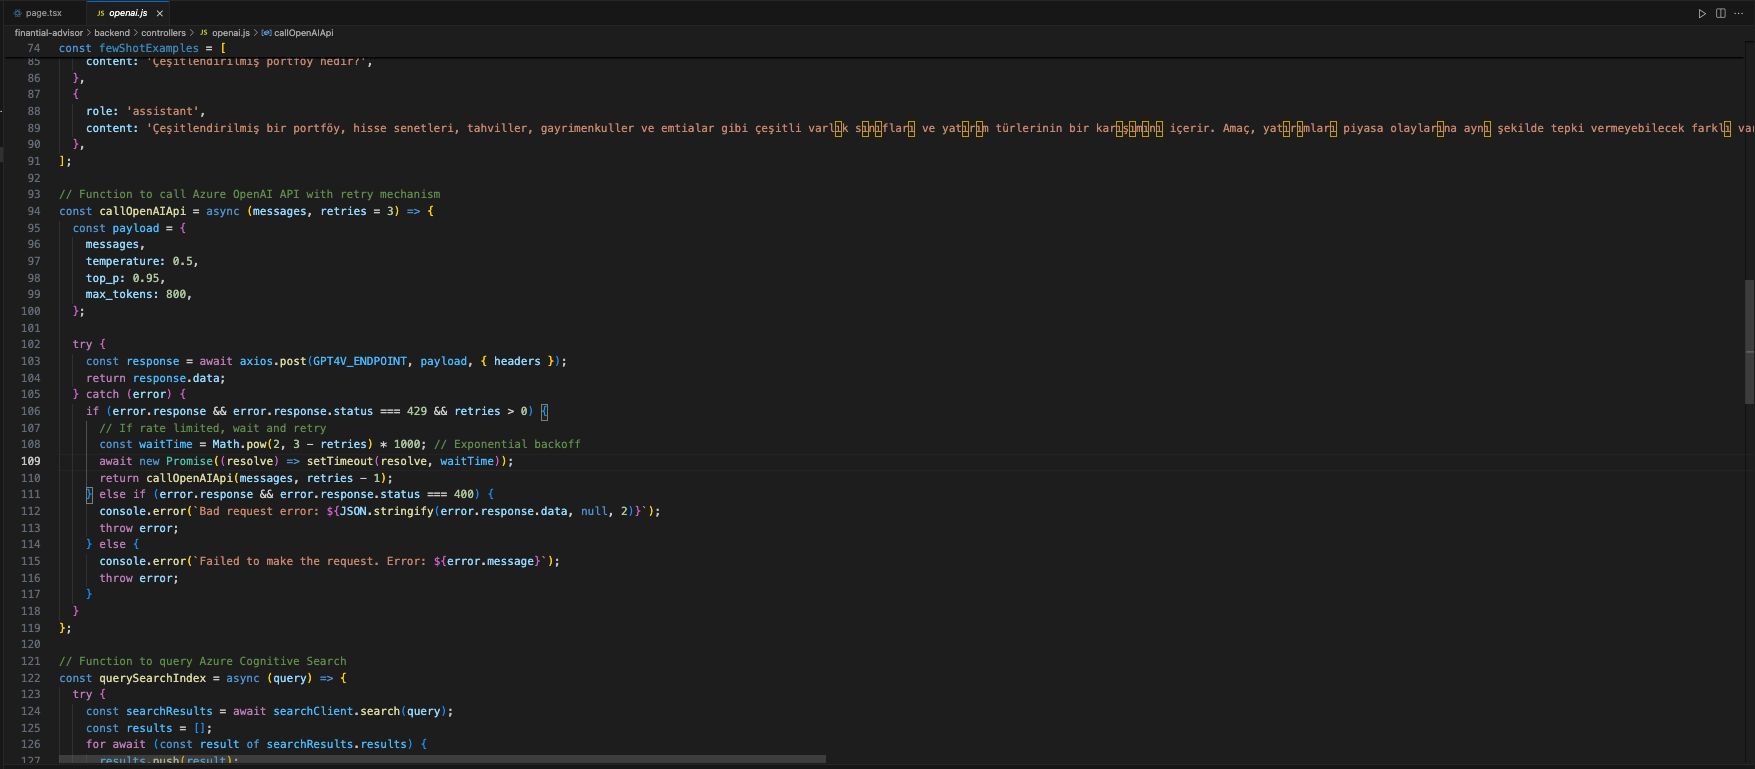
\includegraphics[width=0.8\textwidth]{azure_api.png}
    \caption{API Integration Example in the Backend}
    \label{fig:api-integration}
\end{figure}

\begin{figure}[H]
    \centering
    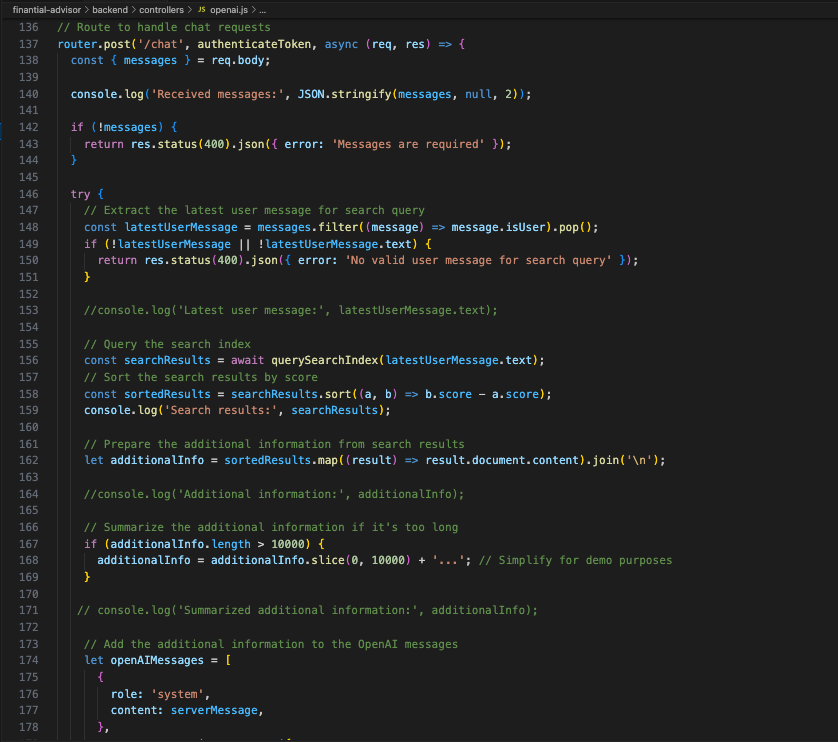
\includegraphics[width=0.8\textwidth]{backend_code.png}
    \caption{Backend Code Written by me for OpenAI Integration}
    \label{fig:api-integration}
\end{figure}

\begin{figure}[H]
    \centering
    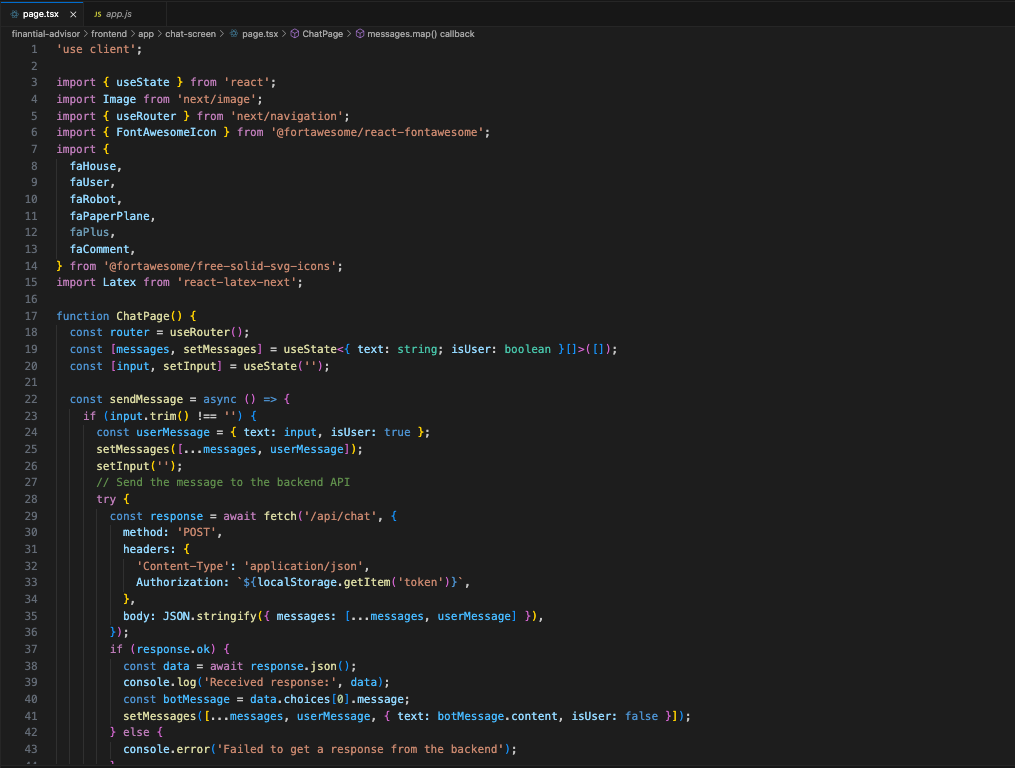
\includegraphics[width=0.8\textwidth]{frontend_code.png}
    \caption{Frontend Code Written by me for Chat Screen}
    \label{fig:api-integration}
\end{figure}

\begin{figure}[H]
    \centering
    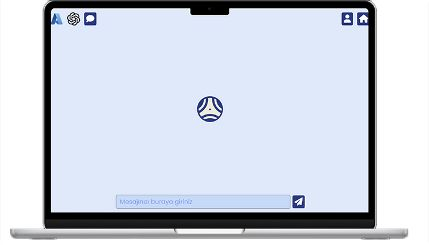
\includegraphics[width=0.8\textwidth]{chatscreen_ui.jpeg}
    \caption{Frontend User Interface for the Chat Screen}
    \label{fig:frontend-ui}
\end{figure}

\begin{figure}[H]
    \centering
    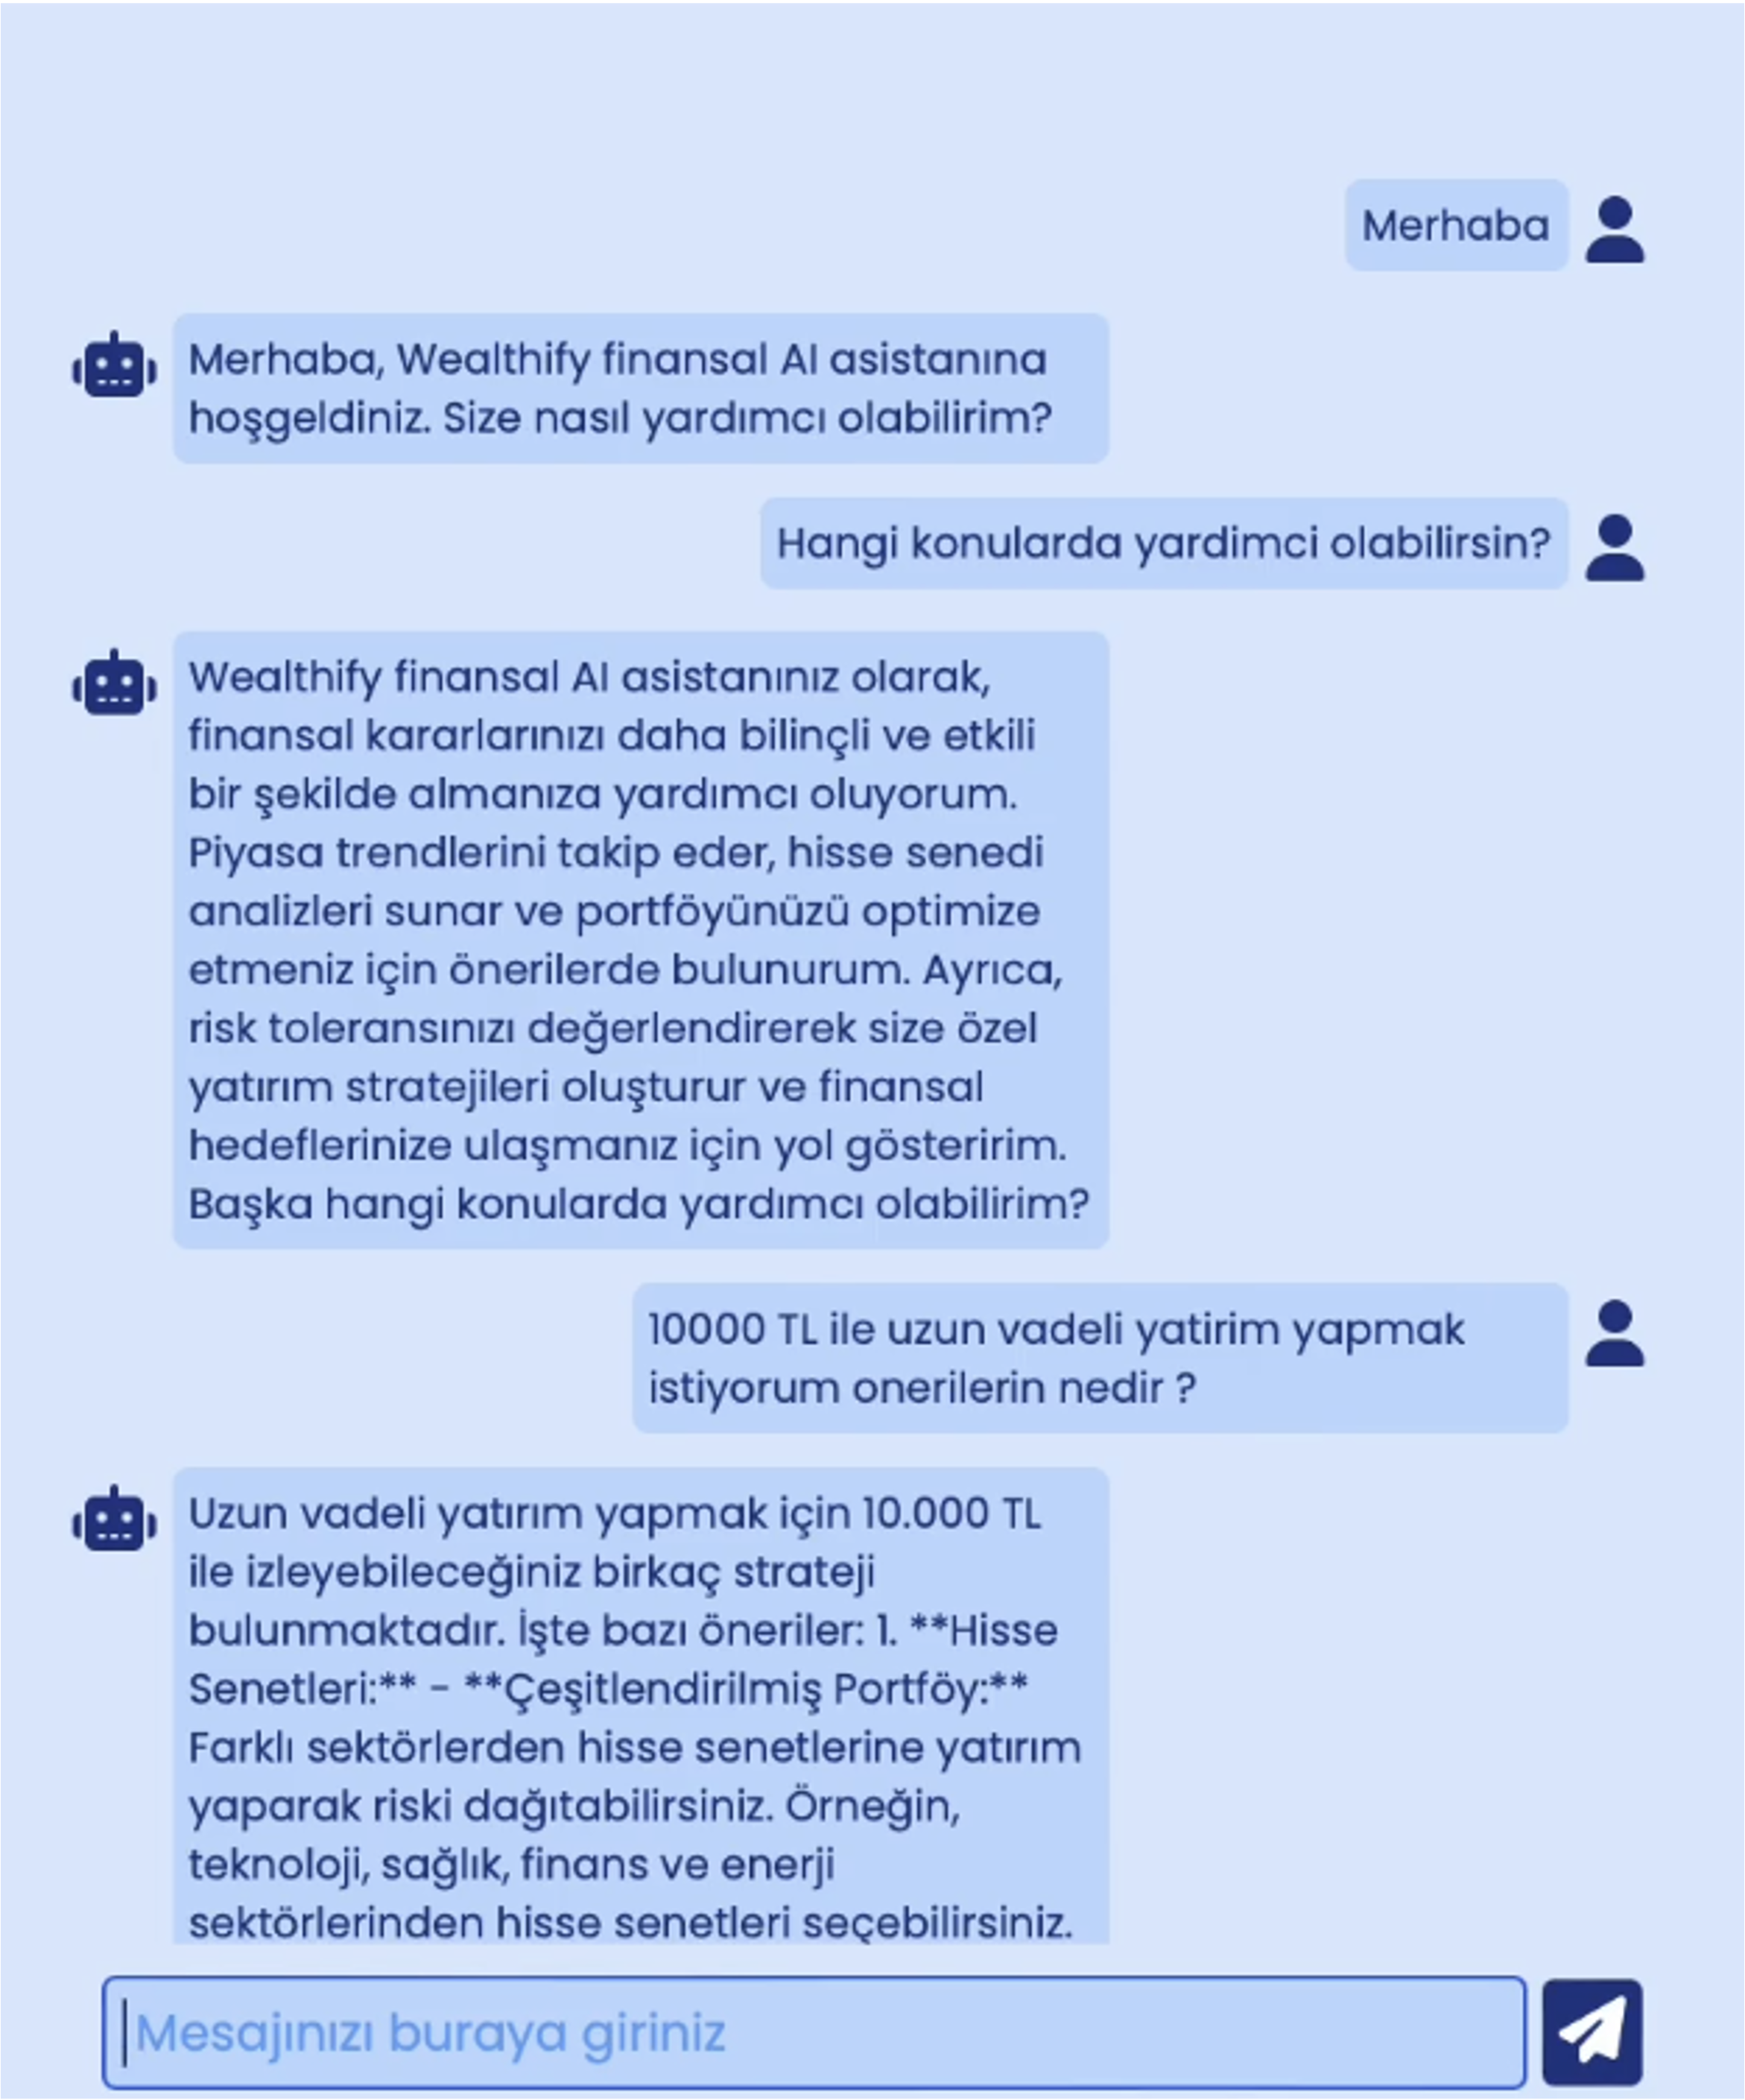
\includegraphics[width=0.8\textwidth]{prompt_example.png}
    \caption{Example of Query Responses}
    \label{fig:prompt-engineering}
\end{figure}


\section{Testing Phase}
The testing phase focused on ensuring that the financial advisor bot met the project requirements and functioned as expected. This involved testing both the backend and frontend components, as well as the accuracy and relevance of the bot's responses to user queries.

\subsection*{Testing Objectives}
The primary objectives of the testing phase were:
\begin{itemize}
    \item To verify the accuracy of the financial data provided by the bot.
    \item To ensure that the bot could handle a wide range of user queries accurately.
    \item To validate the performance and scalability of the system under different conditions, including handling multiple simultaneous users.
    \item To check the usability of the frontend, ensuring that users could easily interact with the bot and understand the responses.
\end{itemize}

\subsection*{Testing Methods}
A variety of testing methods were used to assess the bot’s functionality:
\begin{itemize}
    \item \textbf{Unit Testing:} Unit tests were written to verify that individual components of the backend and frontend functioned correctly. For example, the API integration was tested to ensure it returned accurate data, and the frontend components were tested for proper display and interactivity.
    \item \textbf{Integration Testing:} The bot’s integration with Azure OpenAI services was tested to ensure that the system could handle user queries seamlessly, with responses generated quickly and accurately.
    \item \textbf{Load Testing:} Load testing was performed to evaluate how the bot responded under high usage conditions. We simulated multiple users interacting with the bot at the same time to ensure that it remained responsive and performed within acceptable time limits.
    \item \textbf{User Acceptance Testing (UAT):} A group of potential users tested the bot by asking a wide variety of financial questions. Their feedback helped refine both the bot's responses and the user interface.
\end{itemize}

\subsection*{Challenges in Testing}
The testing phase encountered several challenges:
\begin{itemize}
    \item \textbf{Response Accuracy:} While testing the bot’s responses, we found that some complex financial queries did not generate accurate or relevant responses. This required further refinement of the prompt engineering.
    \item \textbf{Handling Ambiguous Queries:} The bot struggled with ambiguous or unclear user inputs, often generating responses that were not helpful. This necessitated the implementation of a clarification mechanism, where the bot would ask users for more information when it could not fully understand the query.
    \item \textbf{Performance Under Load:} During load testing, the bot’s performance began to degrade when a high volume of users interacted with it simultaneously. This required optimizing the backend code and increasing the system’s resource allocation to handle the additional load.
\end{itemize}


\subsection*{Figures and Screenshots}
This section will include screenshots of the testing environment, sample test cases, and load testing results.

\begin{figure}[H]
    \centering
    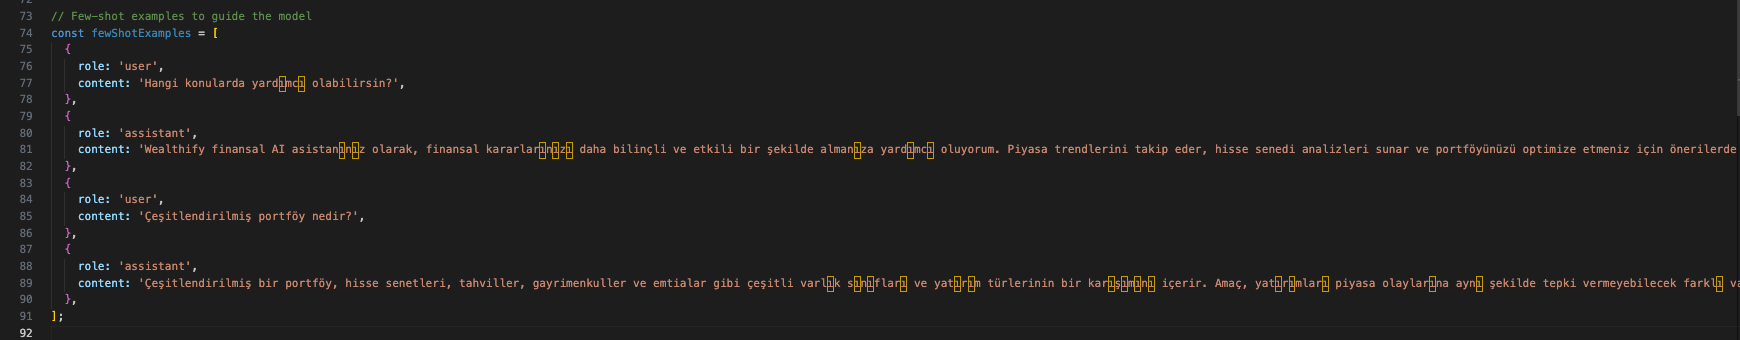
\includegraphics[width=0.8\textwidth]{query_qa.png}
    \caption{Sample Q/A for Financial Query Accuracy}
    \label{fig:test-cases}
\end{figure}

\begin{figure}[H]
    \centering
    \includegraphics[width=0.8\textwidth]{kubernetes.png}
    \caption{Load Testing Results}
    \label{fig:load-testing}
\end{figure}


\chapter{Organization}

\section{Organization and Structure}
Intertech Bilgi İşlem ve Pazarlama Tic. A.Ş is a subsidiary of DenizBank, specializing in providing IT and software development services, particularly in the financial sector. The company plays a crucial role in the digital transformation of financial services, developing cutting-edge software solutions for banking operations, customer service, and financial management.

The project I was involved in was under the Software Development department, specifically focusing on integrating Azure OpenAI services into a financial advisory tool. The team I worked with followed the Agile methodology, which meant we operated in sprints with regular stand-up meetings, sprint reviews, and retrospectives.

\subsection*{Team Structure}
Within the team, there were several key roles:
\begin{itemize}
    \item \textbf{Product Owner:} Responsible for defining the project’s scope, prioritizing features, and ensuring alignment with business goals.
    \item \textbf{Scrum Master:} Facilitated the Agile process and removed any obstacles that could hinder the team's progress.
    \item \textbf{Developers:} Focused on both frontend and backend development, with specific individuals working on API integration, user interface development, and OpenAI prompt engineering.
\end{itemize}

The structure allowed for close collaboration between departments and clear communication channels, which was essential in delivering the project efficiently. The organization encouraged a collaborative work environment where feedback was valued, and continuous improvement was a priority.

\section{Methodologies and Strategies Used in the Organization}
Intertech follows modern software development methodologies, with a strong emphasis on Agile and Scrum frameworks. This approach allows for flexibility in project development, as it breaks the work down into manageable sprints, enabling frequent feedback and adjustments. The core strategies and methodologies employed during my project included:

\subsection*{Agile and Scrum Methodology}
The Agile methodology was central to the organization’s development process. Each sprint typically lasted a week (in our case), during which specific tasks or features were prioritized, developed, and tested. The key principles of Agile that were followed include:
\begin{itemize}
    \item \textbf{Regular Iterations:} By dividing the project into smaller sprints, the team could focus on incremental progress, delivering working software at the end of each sprint.
    \item \textbf{Daily Standups:} Short, daily meetings were held to discuss the progress of each team member, identify blockers, and ensure everyone was aligned with the sprint goals.
    \item \textbf{Sprint Reviews and Retrospectives:} At the end of each sprint, we reviewed the completed work and gathered feedback from stakeholders. Retrospectives allowed the team to reflect on what went well and what could be improved in the next sprint.
\end{itemize}

\subsection*{Tools and Technologies}
To support the Agile framework, Intertech employed several tools and technologies to streamline project management and collaboration:
\begin{itemize}
    \item \textbf{Jira:} This was the primary tool used for managing sprints, tracking tasks, and monitoring progress. Each task was assigned to a team member, and its status was updated throughout the sprint. But we have not used this
    \item \textbf{Git} Git was used for version control, . All code changes were reviewed and merged via pull requests, ensuring that the codebase remained stable.
\end{itemize}

\subsection*{Innovation and Continuous Learning}
One of the key strategies employed at Intertech is a focus on continuous learning and innovation. The company encourages its employees to stay updated with the latest trends in technology and regularly holds internal training sessions. For example, as part of the onboarding process, we received training on the company’s specific tools and best practices.

This focus on learning not only benefits individual employees but also ensures that the company remains competitive in the fast-evolving financial technology landscape. The integration of Azure OpenAI into the project was an example of how Intertech leverages emerging technologies to innovate and deliver superior solutions.

\subsection*{Team Collaboration and Communication}
Throughout the project, collaboration and communication were key elements that contributed to its success. Regular meetings with stakeholders, both internal and external, ensured that everyone was aligned with the project goals. The use of tools like Mural and Slack facilitated efficient communication and task tracking, while daily standups ensured that any issues were addressed promptly.


% Section 4: Conclusion
\chapter{Conclusion}
The summer practice at Intertech Bilgi İşlem ve Pazarlama Tic. A.Ş provided invaluable hands-on experience in software development, project management, and teamwork within the context of the financial technology industry. Through my work on the financial advisor bot, I had the opportunity to apply both technical and analytical skills, gaining deep insights into the integration of artificial intelligence with real-time financial data.

One of the key takeaways from this experience was the importance of collaboration in a fast-paced, Agile-driven environment. Working in a multidisciplinary team allowed me to understand different perspectives, from the technical challenges of backend and frontend development to the broader business goals addressed by the product owner. The Agile methodology, with its iterative process, facilitated continuous feedback and improvement, ultimately leading to a more refined and user-friendly product.

The financial advisor bot project presented several challenges, particularly in the areas of prompt engineering, API integration, and real-time data handling. However, these challenges provided valuable learning opportunities, allowing me to develop problem-solving strategies that I can apply to future projects. The ability to quickly adapt to changing requirements and improve the bot’s functionality through testing and refinement was a critical aspect of the project’s success.

This summer practice also reinforced the importance of innovation and continuous learning in the rapidly evolving field of financial technology. The training sessions broadened my knowledge and helped me stay up-to-date with the latest tools and technologies. The project itself, with its use of Azure OpenAI services, demonstrated how cutting-edge technologies can be harnessed to improve financial services and enhance customer experience.

In conclusion, this internship not only helped me enhance my technical skills in software development and artificial intelligence but also gave me a solid understanding of how a large organization like Intertech operates within the financial sector. The experience of working on a real-world project from start to finish, collaborating with team members, and seeing the impact of my contributions has been highly rewarding. I am confident that the skills and knowledge gained during this summer practice will serve as a strong foundation for my future career in the field of computer engineering.

\subsection*{Future Improvements and Reflection}
Looking back, there are areas where the project could be further enhanced. For instance, future iterations of the financial advisor bot could incorporate more advanced natural language processing techniques to handle even more complex financial queries. Additionally, further optimization of the backend infrastructure could improve scalability, enabling the bot to handle a greater number of simultaneous users.

This reflection on the project has been crucial in helping me recognize my growth over the summer practice. Moving forward, I aim to apply the skills I’ve developed in new projects and continue learning to stay ahead of technological trends in the industry.

\subsection*{Figures and Screenshots}
To complement this conclusion, I will include final diagrams and summary screenshots of the project's key components, such as the final user interface of the bot.

\begin{figure}[H]
    \centering
    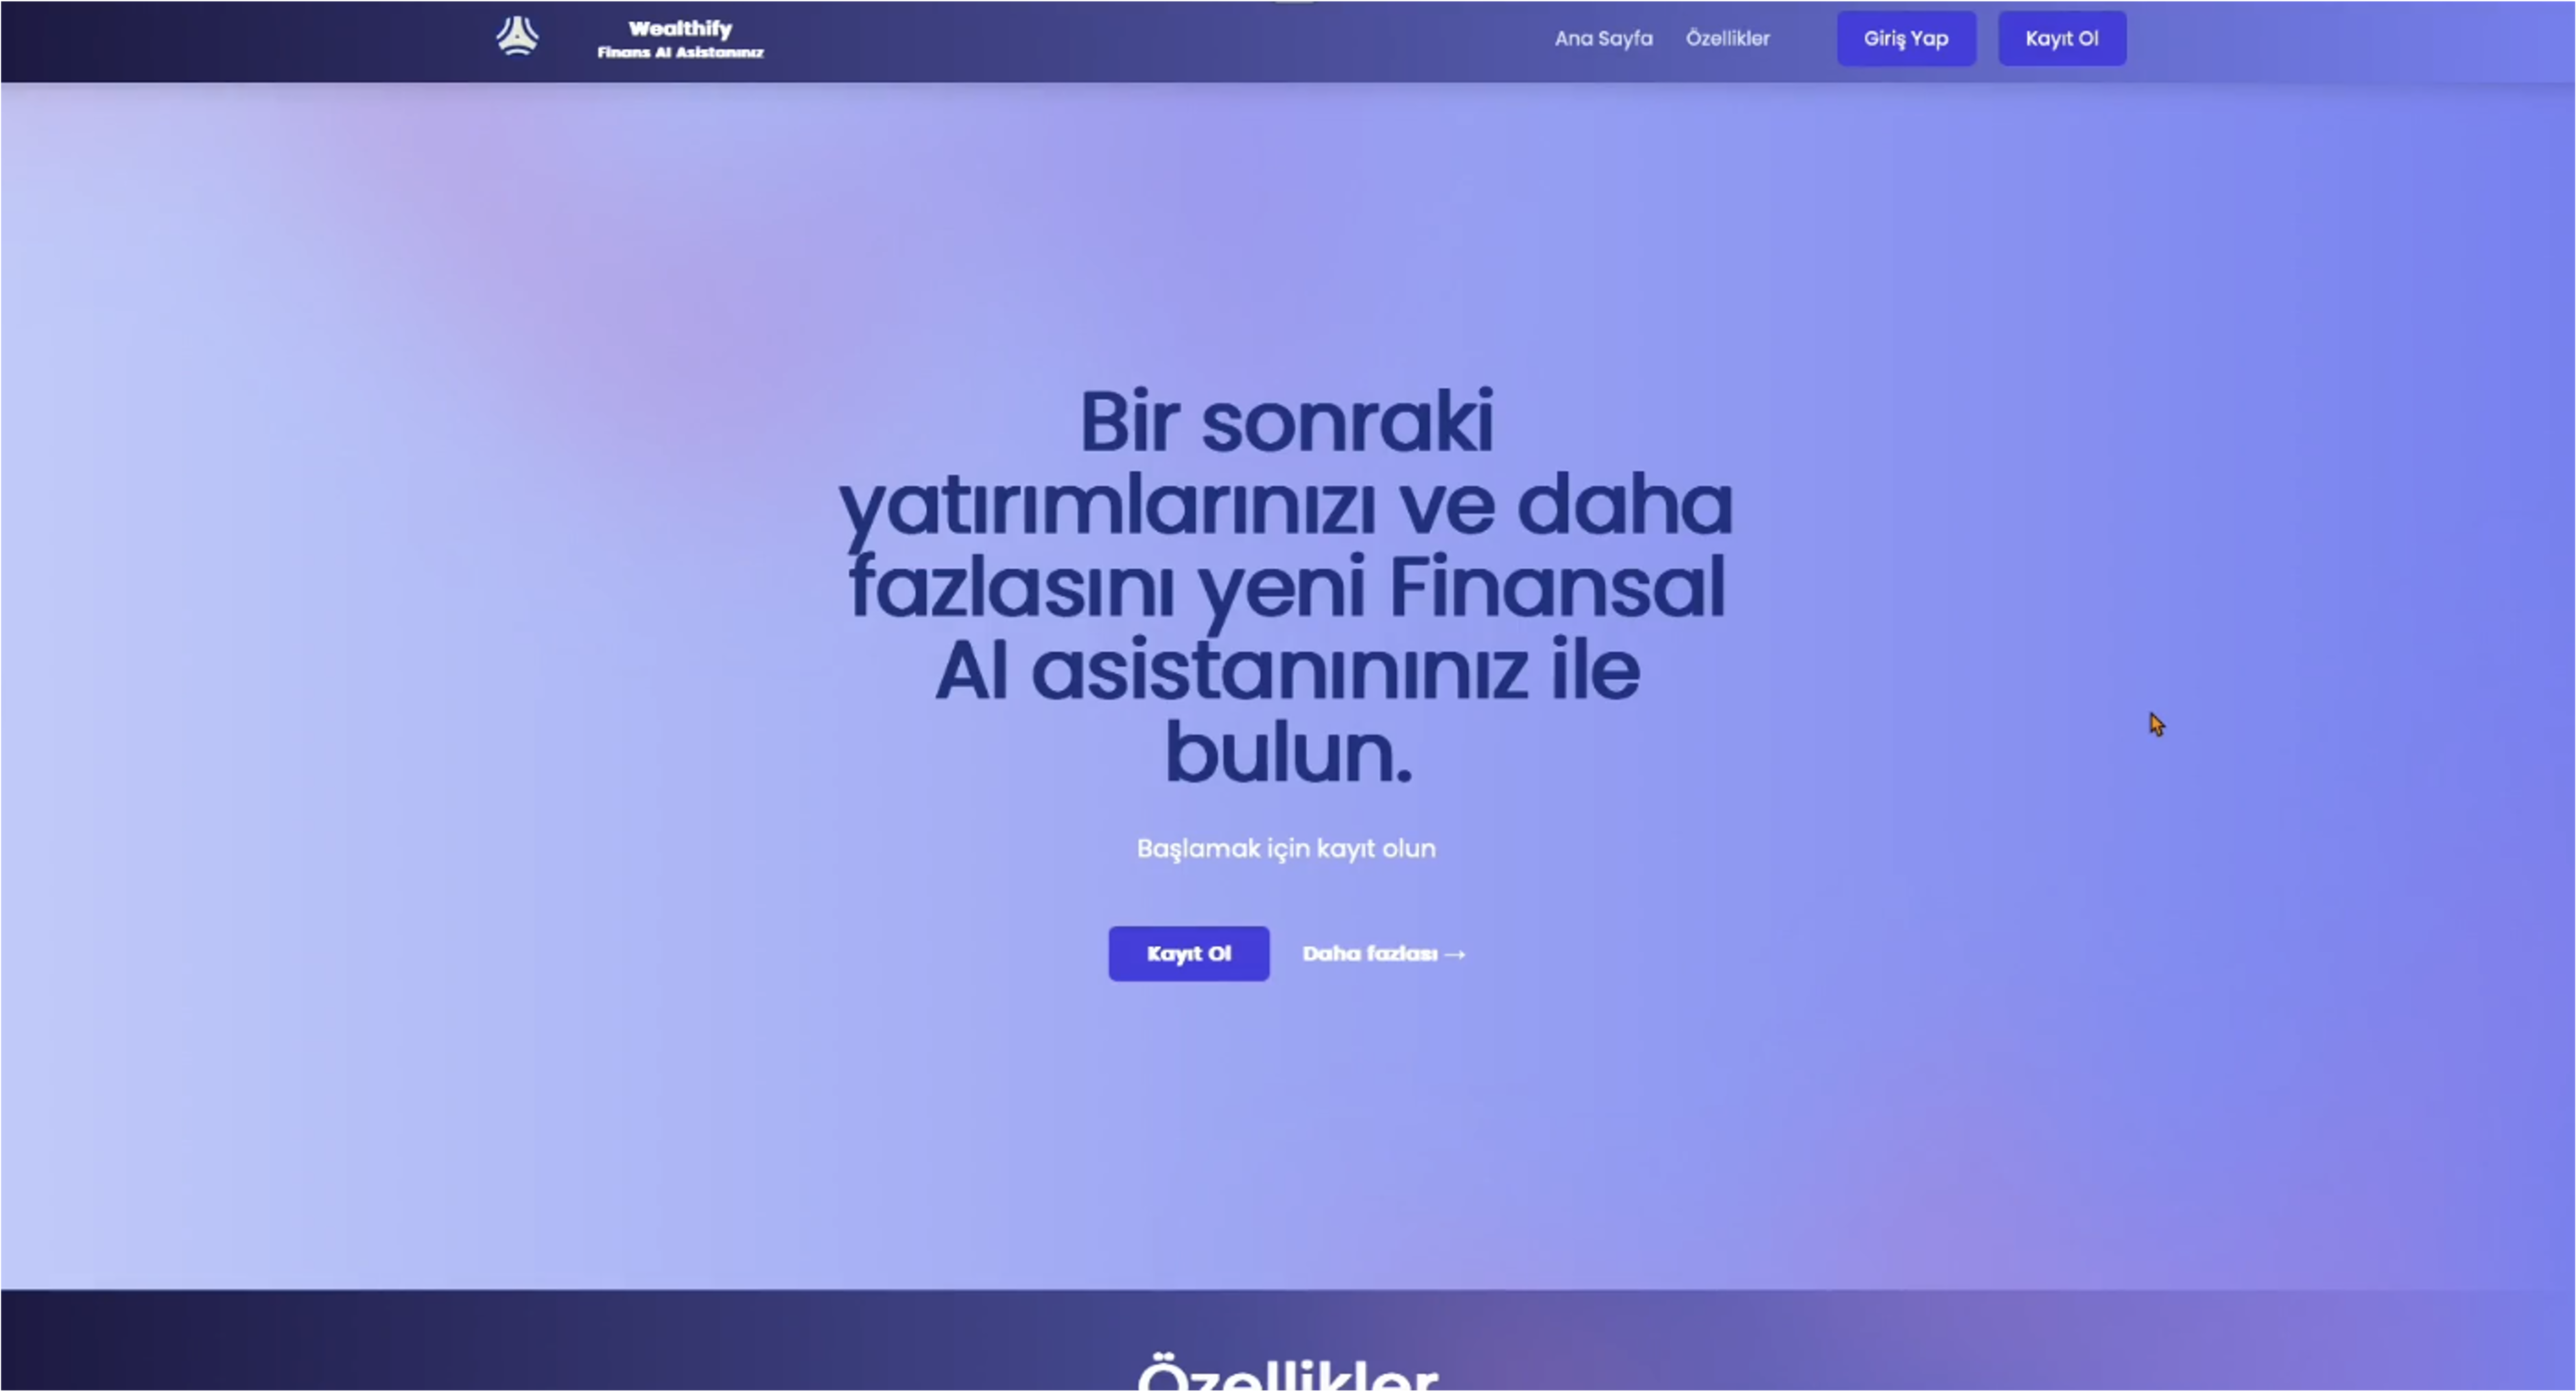
\includegraphics[width=0.8\textwidth]{ui_homepage.png}
    \caption{Final User Interface Design of Homepage}
    \label{fig:final-ui-design}
\end{figure}

\begin{figure}[H]
    \centering
    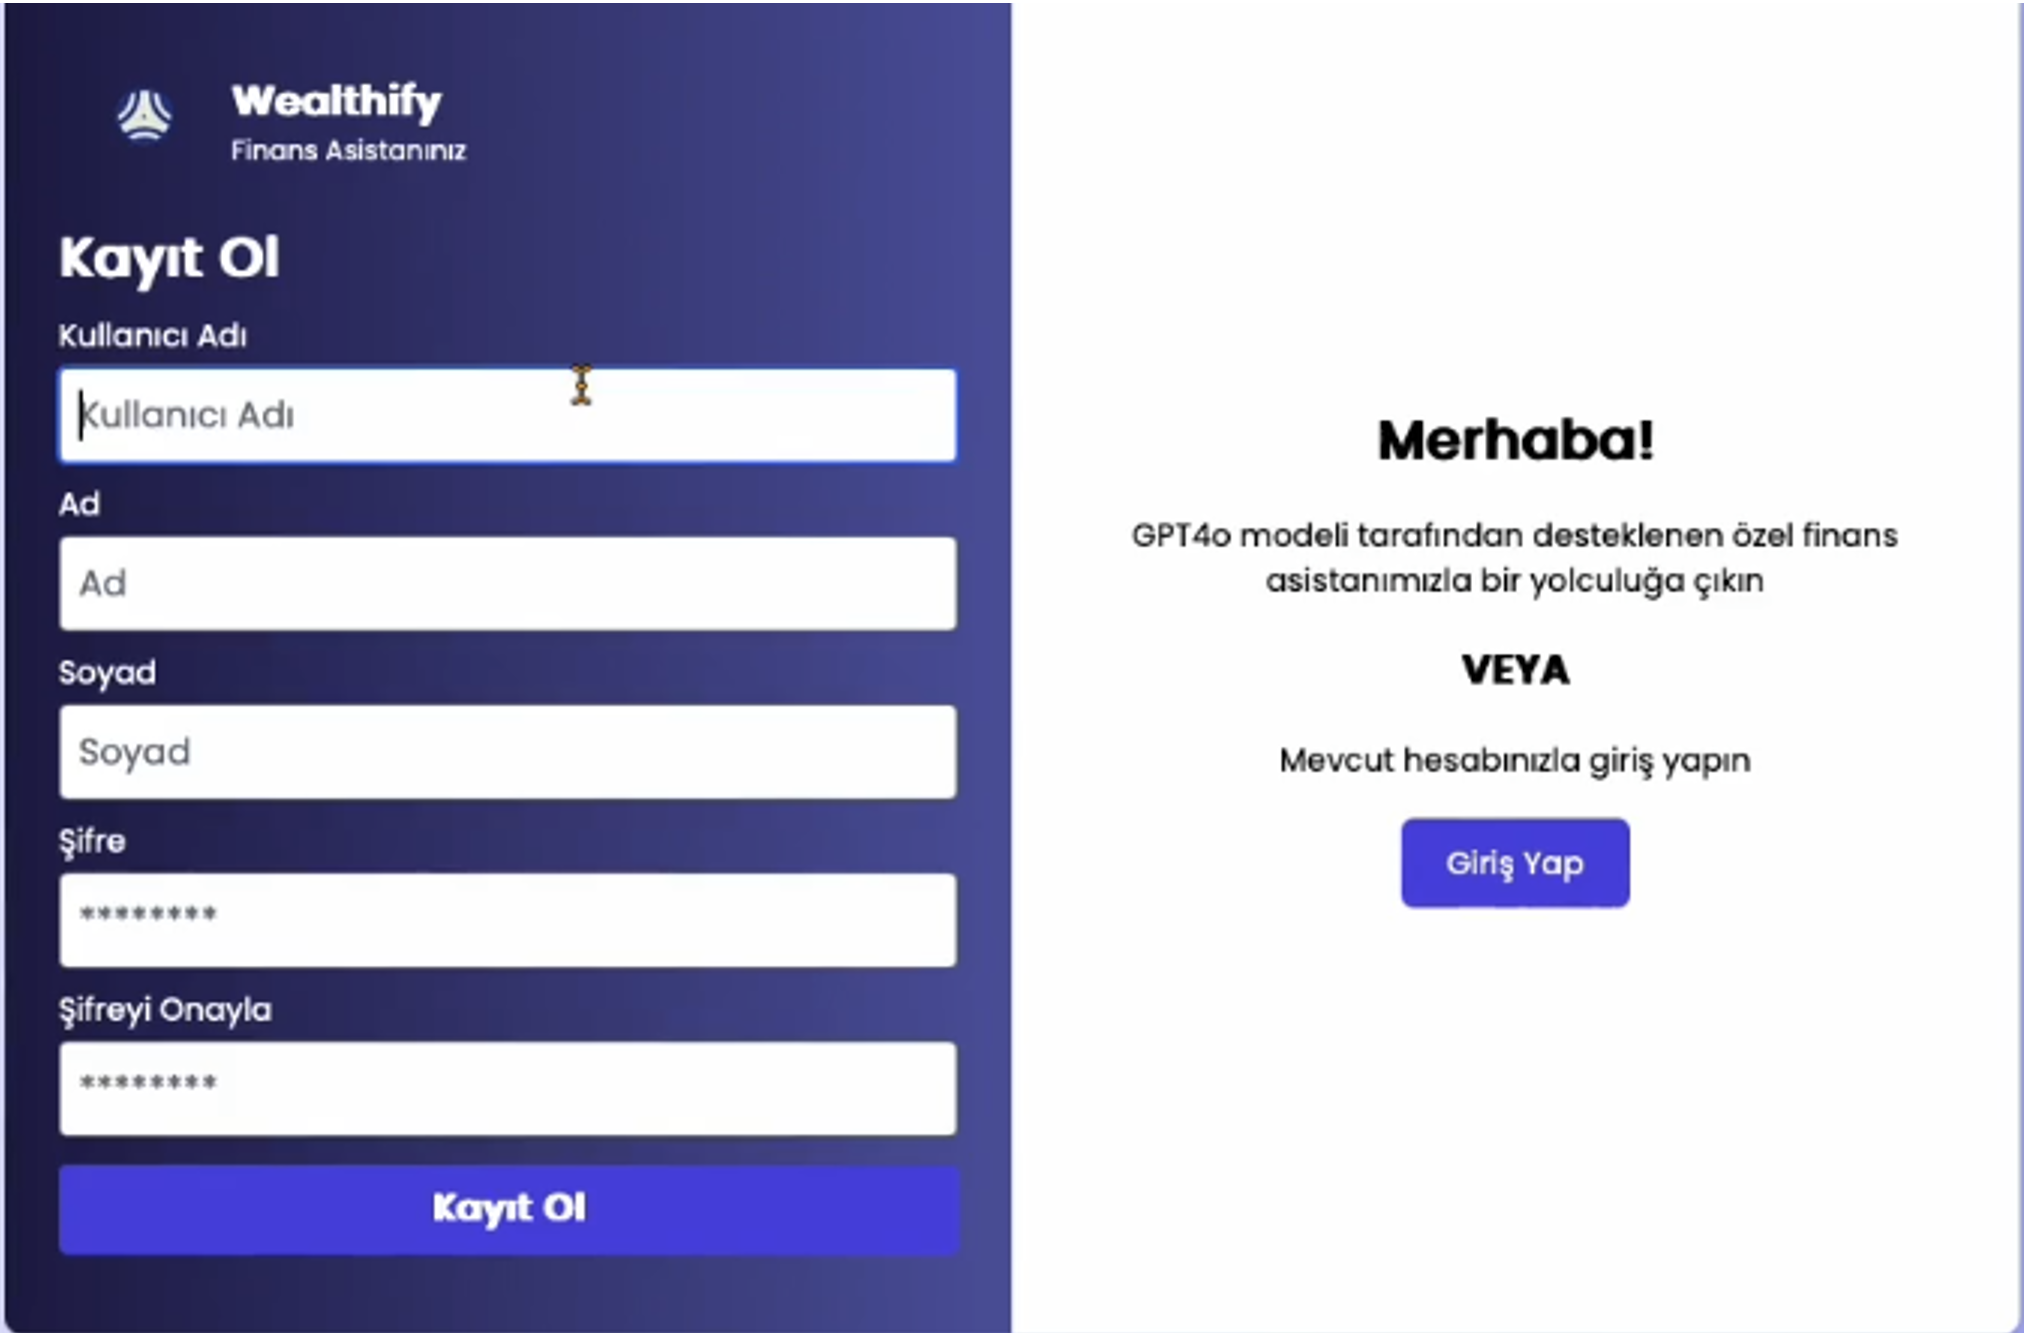
\includegraphics[width=0.8\textwidth]{ui_register.png}
    \caption{Final User Interface Design of Register Page}
    \label{fig:final-ui-design}
\end{figure}

\begin{figure}[H]
    \centering
    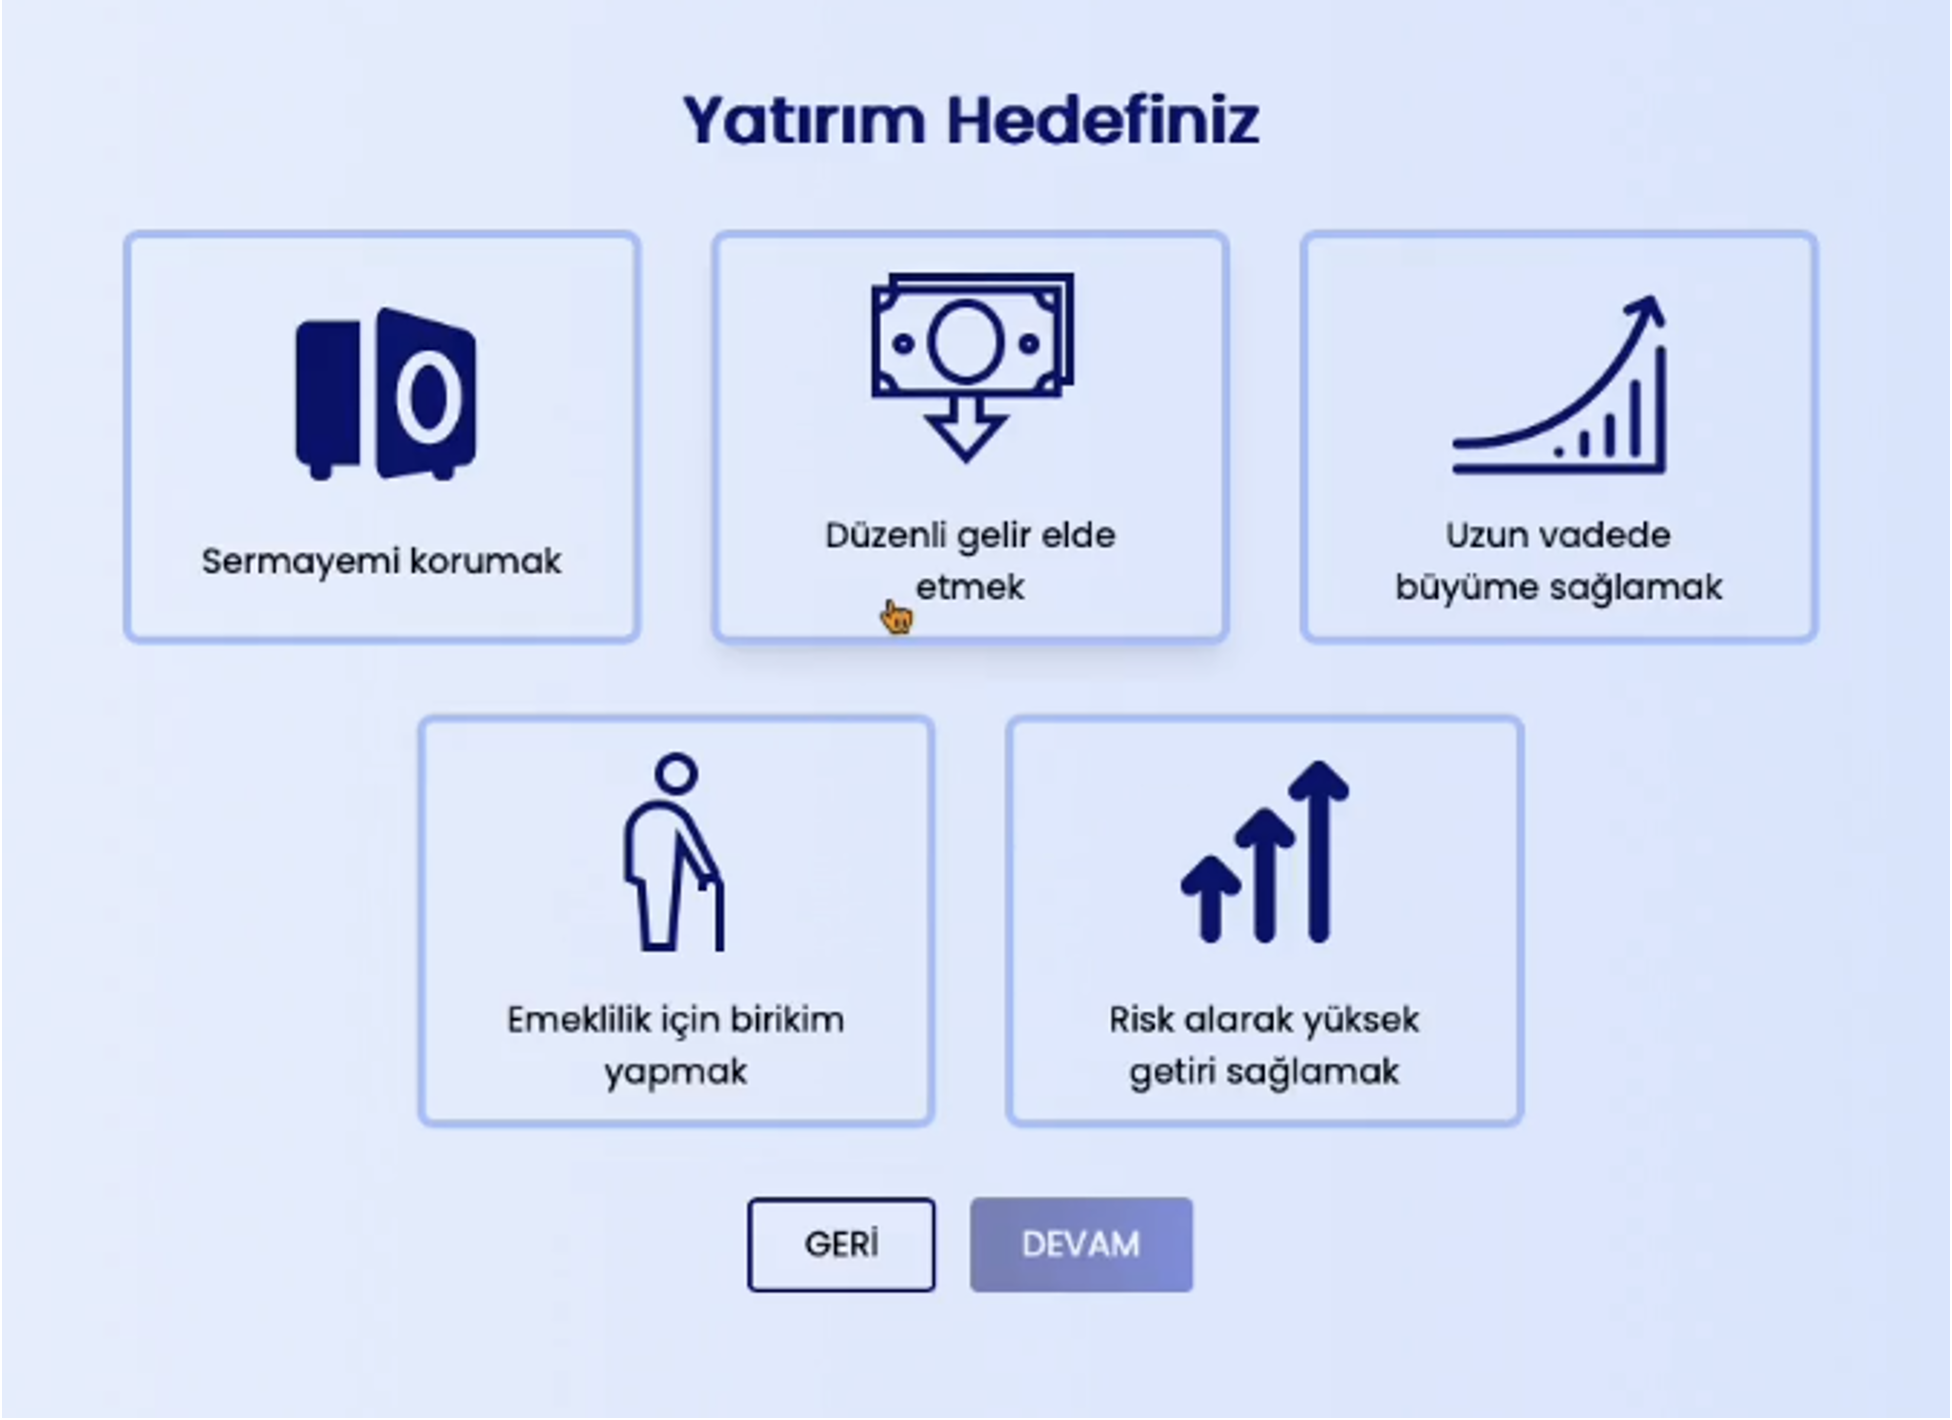
\includegraphics[width=0.8\textwidth]{ui_test.png}
    \caption{Final User Interface Design of the Analysis Test}
    \label{fig:final-ui-design}
\end{figure}



\end{document}
